\chapter{The Polar Front as a major biogeographic boundary in the Southern Ocean} 
\label{ch:polarfront}

\emph{Sections of this chapter have been previously published in (TODO: cite PF manuscript)}

\section{Summary}

\section{Introduction}


\section{Methods}
\subsection{Sampling and metagenomic sequencing}

Sampling\footnote{Sampling was performed by Jeffrey M. Hoffman and Jeffrey B. Mcquaid} was conducted on board the RSV \emph{Aurora Australis} during cruise V3 CEAMARC/CASO (Collaborative East Antarctic Marine Census / Climate of Southern Ocean) from 13 December 2007 -- 26 January 2008. 
This cruise occupied the SR3 latitudinal transect from Hobart, Australia (44$^\circ$ S) to the Mertz Glacier, Antarctica (67$^\circ$ S) within a longitudinal range of 140--150$^\circ$ E.
Nineteen samples (16 surface, 3 deep) were obtained along almost the entire latitudinal range \figref{fig:samplemap}.

% the sample map
\begin{figure}[!ht]
  \centering
  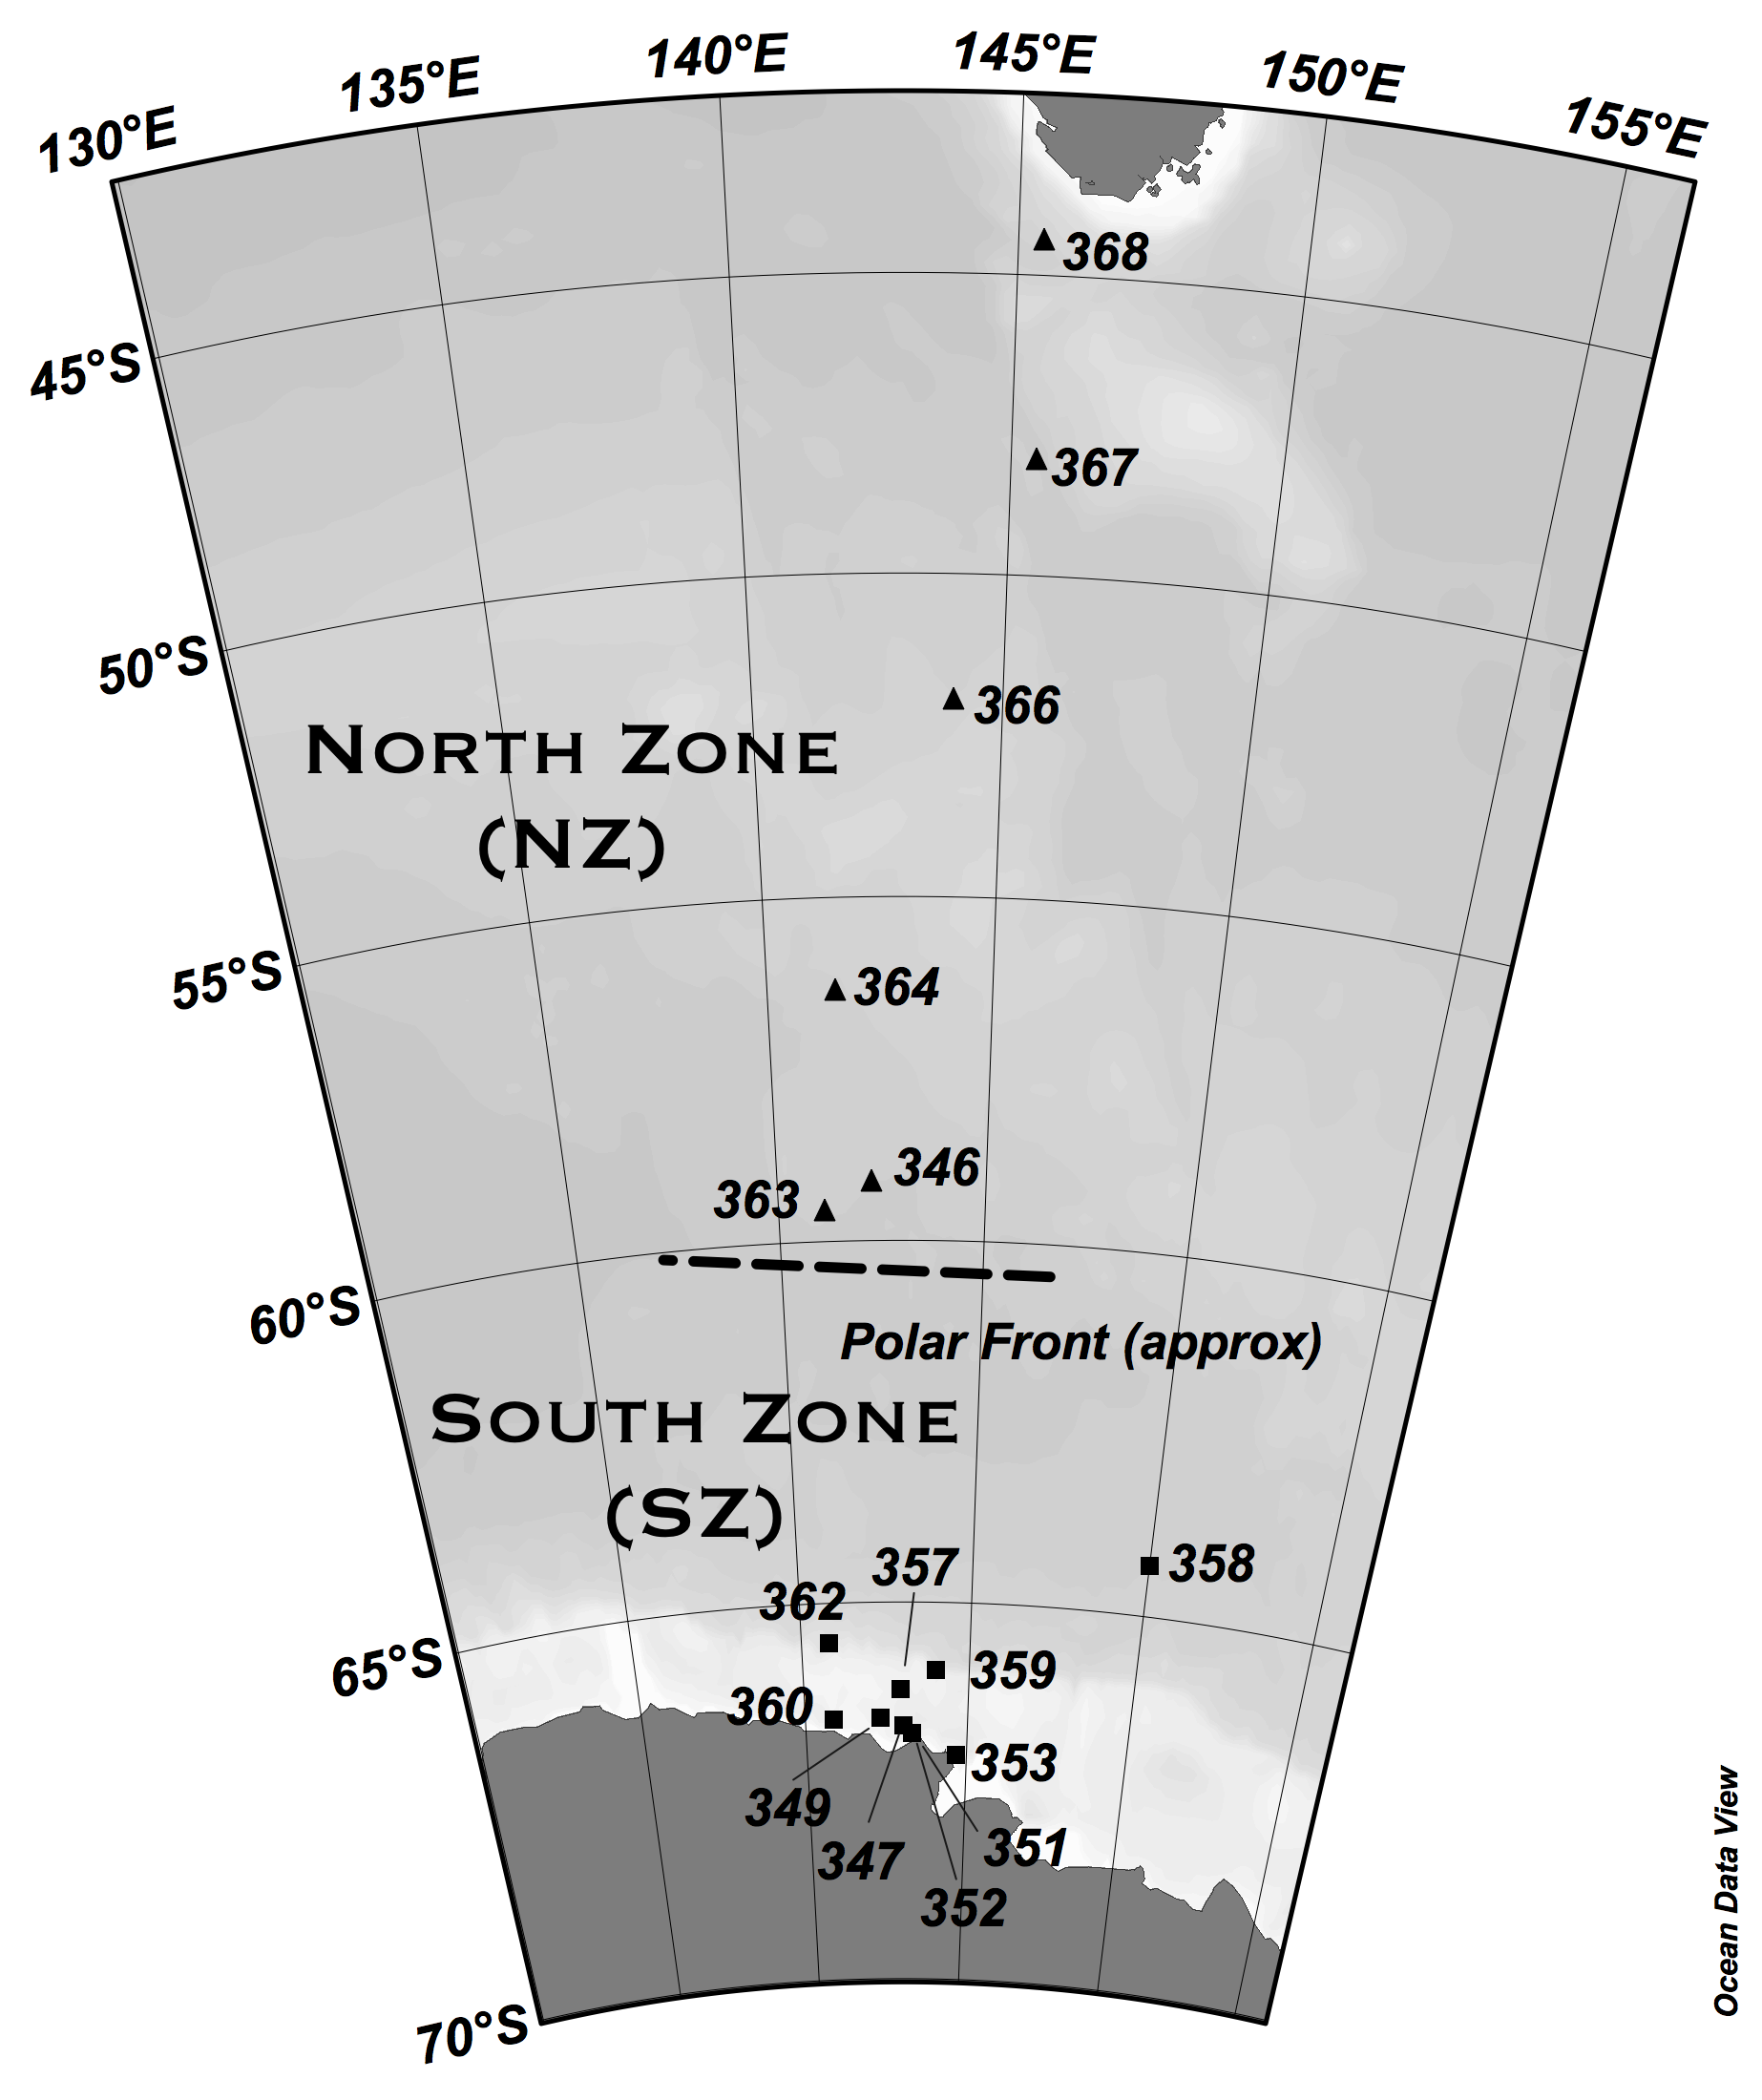
\includegraphics[width=\textwidth]{../polarfront/samplemap.png}
  \caption[Map showing sites of seawater samples used in the Polar Front study]{Sites of seawater samples used in this study. 
  Squares indicate surface samples from the North Zone; crosses samples from the South Zone. 
  The dashed line represents the Polar Front.}
  \label{fig:samplemap}
\end{figure}


At each station, $\sim$ 500 L of seawater was pumped from $\sim$ 2 m below the sea surface into drums stored at ambient temperature on deck. 
In the case of deep samples, $\sim$ 10--50 L of seawater was collected opportunistically from Niskin bottles attached to a CTD (Conductivity, Temperature and Depth) instument operated by an unrelated oceanographic project.
Seawater samples were prefiltered through a 20 $\mu$m plankton net, then filtrate was captured on sequential 3.0 $\mu$m, 0.8 $\mu$m and 0.1 $\mu$m polyethersulfone membrane filters (Supor membrane disc filter; Pall Life Sciences), and immediately stored at $-20$ $^\circ$C \cite{Rusch:2007ez,Ng:2010cd}.


\subsection{Phylogenetic analysis of metagenomic data}
\subsection{Functional analysis of metagenomic data}

\section{Results}
\subsection{Metagenomic sequencing}
\subsection{Phylogenetic analysis of metagenomic data}
\subsection{Functional analysis of metagenomic data}

\section{Discussion}

\section{Conclusions}

